\documentclass{beamer}
\usetheme{Madrid}
\usepackage{lmodern}
\usepackage{hyperref}
\usepackage{apacite}
\usepackage[utf8]{inputenc}
\usepackage[spanish]{babel}

\usepackage{xcolor}
\setbeamertemplate{background}{\tikz[overlay,remember picture]\node[opacity=0.2]at (current page.center){
\includegraphics[width=13cm]{KL.png}};}
\usepackage{tikz}
\usepackage{kantlipsum}

\setbeamercolor{normal text}{fg=black}

\begin{document}
\colorlet{beamer@blendedblue}{blue!46!green}
\setbeamercolor{normal text}{fg=black}

\setbeamercolor{frametitle}{fg=white, bg=blue!46!green}
\setbeamercolor*{title}{bg=blue!46!green, fg=white}

\setbeamercolor{section in toc}{fg=black}

\author[Juan C. Correa \textcolor{white}{(\url{https://correajc.com}})]{Juan C. Correa, Ph.D.}
\title[Enseñanza basada en reproducibilidad]{Enseñanza basada en reproducibilidad}
% \subtitle{TREME}
	%\subtitle{}
\institute[]{Fundación Universitaria Konrad Lorenz\\
	\color{blue}\Email  \href{mailto:juanc.correan@konradlorenz.edu.co}{juanc.correan@konradlorenz.edu.co}}
\pgfdeclareimage[height=0.5cm]{KL}{KL}
\logo{\pgfuseimage{KL}}
\setbeamertemplate{caption}[numbered]
\date[Bogotá, Junio-2021]{Curso en: \textbf{T}ecnologías \textbf{R}eproducibles en la \textbf{E}nseñanza de la \textbf{M}etodología y la \textbf{E}stadística}

%\subject{}
\setbeamercolor{background canvas}{bg=white}
%\setbeamertemplate{navigation symbols}{}

\begin{frame}
	\titlepage
\end{frame}

\begin{frame}
\begin{block}{Objetivo del Curso}
\vspace{0.3cm}
Comprender, a través de ejemplos concretos, los beneficios de usar repositorios de datos públicos para la enseñanza de contenidos metodológicos y estadísticos.  
\end{block}
\end{frame}



\begin{frame}
\frametitle{Agenda} 
\tableofcontents
\end{frame}

\section{El por qué de los repositorios de datos}
\begin{frame}{Repositorios de datos ¿Por qué?}
\tiny{\textcolor{blue}{\url{https://www.researchgate.net/publication/6763307_The_poor_availability_of_psychological_research_data_for_reanalysis}}}
\begin{figure}
\centering

\includegraphics[width=0.8\textwidth]{psycdata}
\end{figure}
\end{frame}

\begin{frame}{Repositorios de datos ¿Por qué?}
\begin{figure}
\centering

\includegraphics[width=0.4\textwidth]{codingr}
\end{figure}
Iniciativas como GitHub o Stackoverflow (fundadas en 2008) visibilizaron los beneficios pedagógicos de compartir conocimientos aplicados para el  desarrollo de software en ramas como la estadística, la genética, la manufactura, el control de procesos, etc.
\end{frame}

\begin{frame}{Repositorios de datos ¿Por qué?}
\textcolor{blue}{\url{https://www.redalyc.org/pdf/727/72711895025.pdf}}
\begin{figure}
\centering
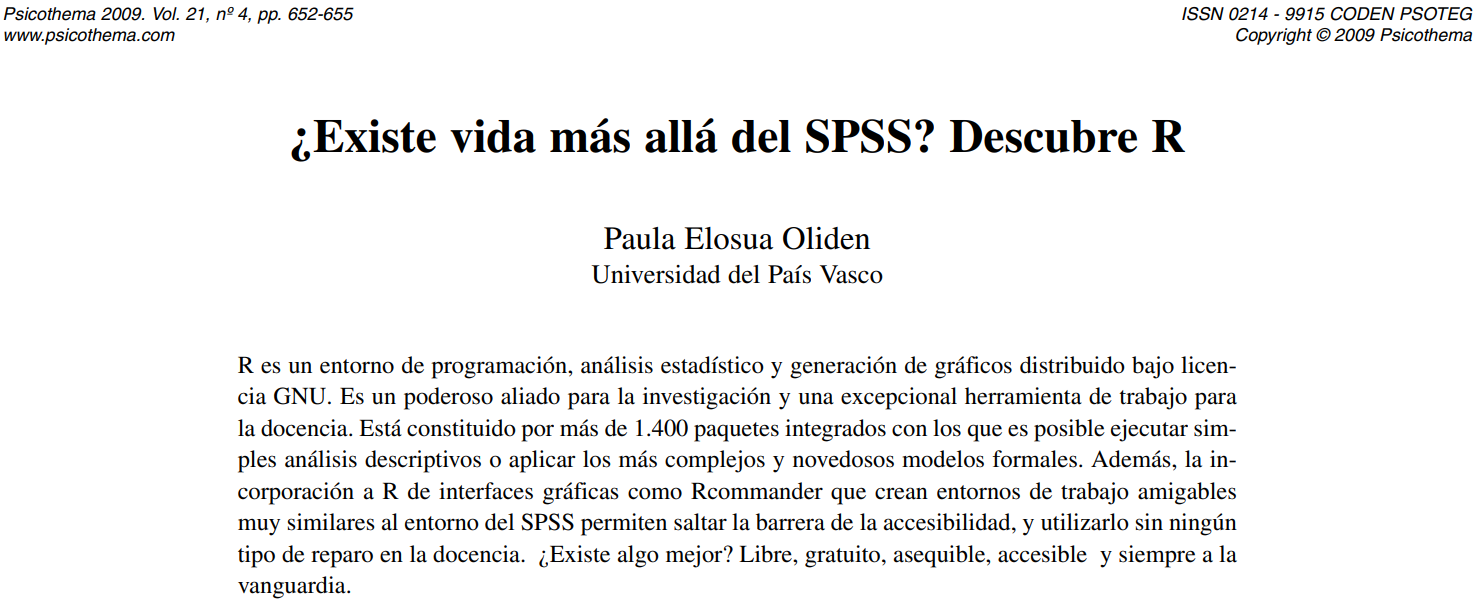
\includegraphics[width=1\textwidth]{RSPSS.png}
\end{figure}
Iniciativas como GitHub o Stackoverflow facilitaron la popularización de software y datos abiertos.
\end{frame}

\section{Repositorios de datos}
\begin{frame}{Repositorios de datos}
Un repositorio de datos abarca a un conjunto de recursos de hardware y/o software donde se almacenan conjuntos de datos estructurados (numéricos, geoespaciales, textuales, audiovisuales, o de cualquier otro formato) para su uso secundario con fines de investigación o docencia.
\end{frame}

\begin{frame}{Repositorios de datos}
Algunos repositorios de datos disponibles:
\begin{itemize}
\item En Ciencias Naturales
\begin{itemize}
    \item \url{https://rda.ucar.edu/}
    \item \url{https://datadryad.org/stash}
    \item \url{http://archive.eso.org/cms.html}
    \item \url{https://www.dataone.org/}
    \item \url{https://figshare.com/}
\end{itemize}
\item En Ciencias Sociales
\begin{itemize}
    \item \url{https://www.icpsr.umich.edu/web/pages/}
    \item \url{https://www.re3data.org/}
    \item \url{https://ciser.cornell.edu/data/data-archive/}
    \item \url{https://dataverse.harvard.edu/}
    \item \url{https://www.europeansocialsurvey.org/}
\end{itemize}
\end{itemize}
\end{frame}

\section{Algunos Ejemplos}
\subsection{Psicología de la corrupción y la riqueza}
\begin{frame}{Psicología de la corrupción y la riqueza}
\begin{figure}
\centering
 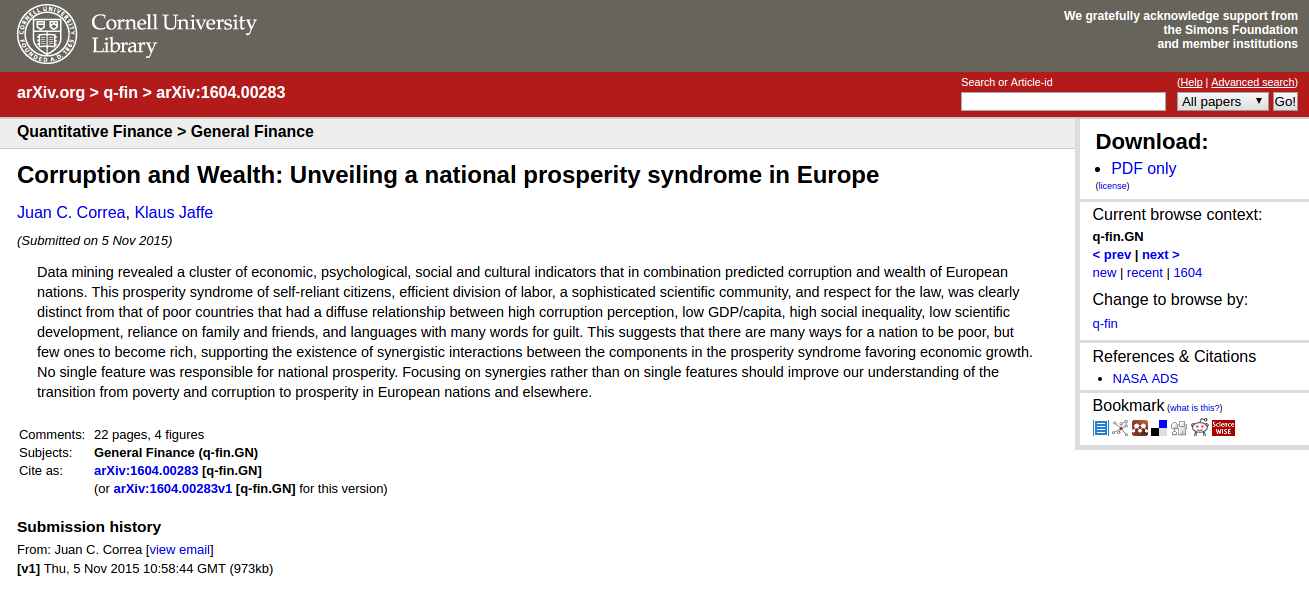
\includegraphics[width=1\textwidth]{Case_1}
 \end{figure}
 \textcolor{blue}{\url{https://arxiv.org/abs/1604.00283}}
 \end{frame}

\begin{frame}{Psicología de la corrupción y la riqueza}
\begin{figure}
\centering
 
\includegraphics[width=0.8\textwidth]{data}
 \end{figure}
\end{frame}

\begin{frame}{Psicología de la corrupción y la riqueza}
\begin{figure}
\centering
 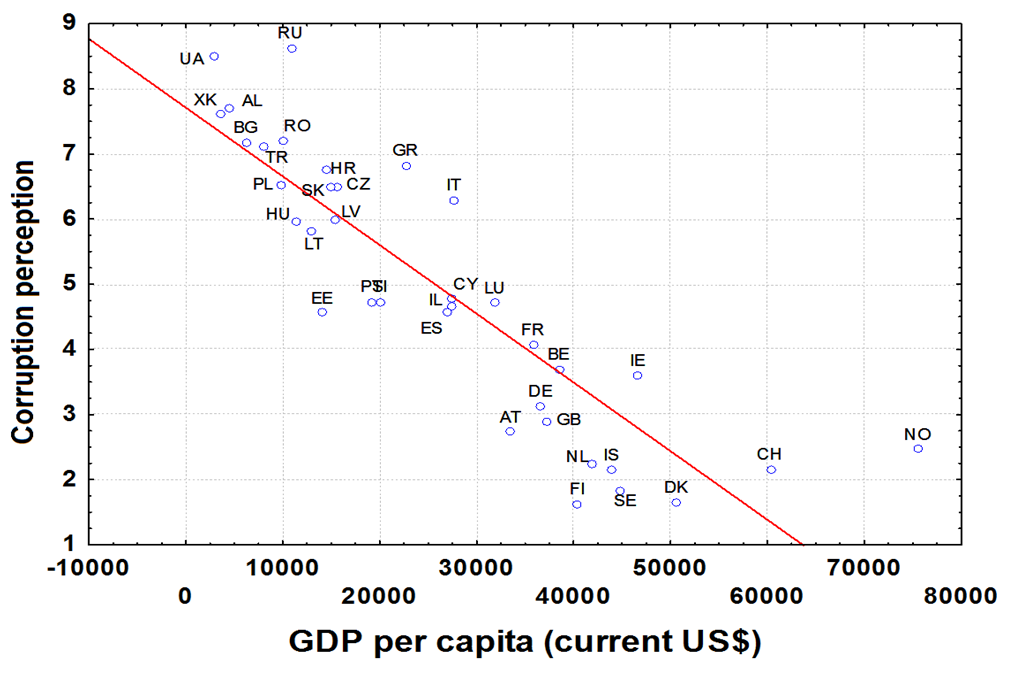
\includegraphics[width=0.85\textwidth]{F1}
 \end{figure}
\end{frame}

\begin{frame}{Psicología de la corrupción y la riqueza}
\begin{figure}
\centering
 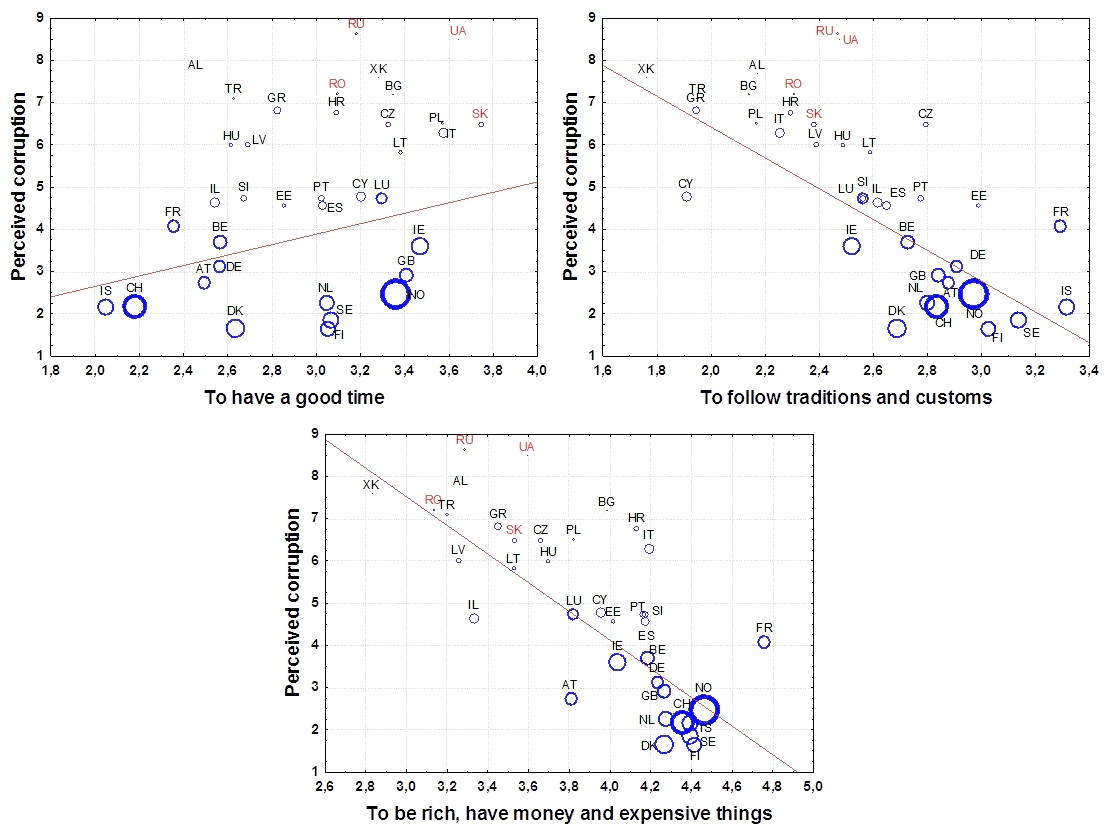
\includegraphics[width=0.85\textwidth]{F2}
 \end{figure}
\end{frame}

\begin{frame}{Psicología de la corrupción y la riqueza}
\begin{figure}
\centering
 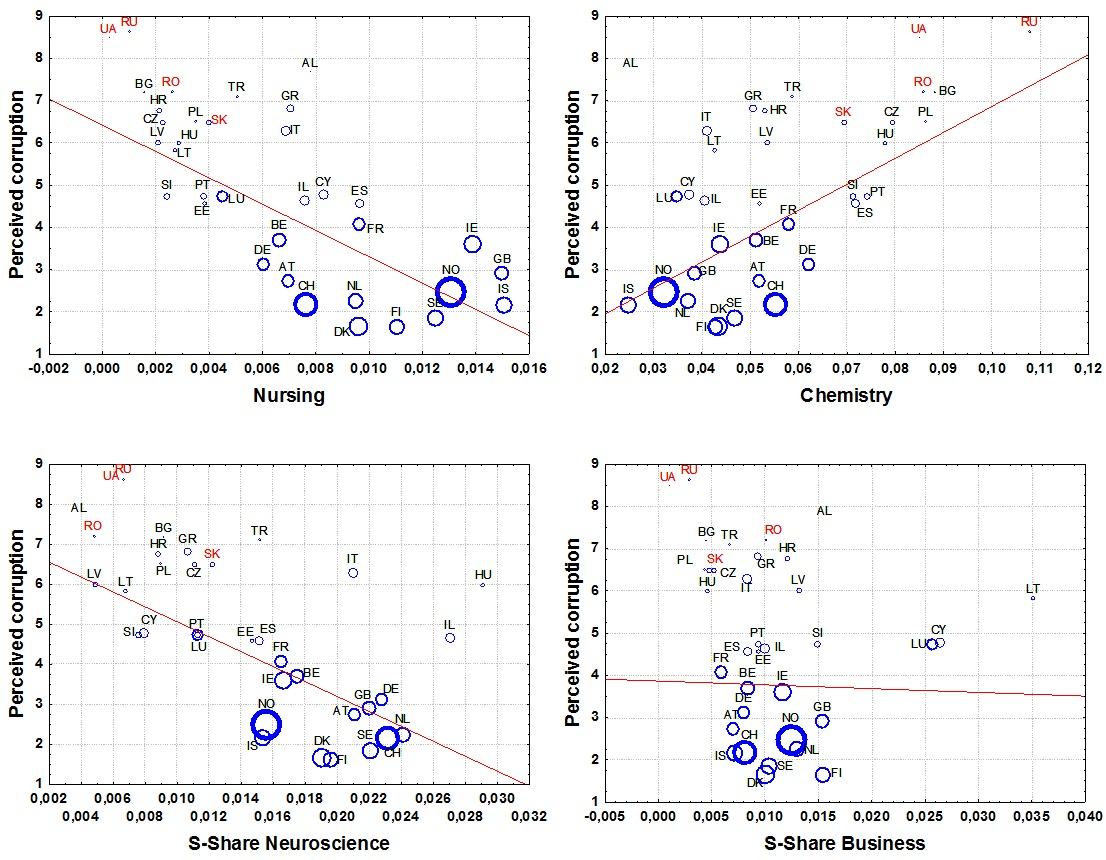
\includegraphics[width=0.85\textwidth]{F3}
 \end{figure}
\end{frame}

\begin{frame}{Psicología de la corrupción y la riqueza}
\begin{figure}
\centering
 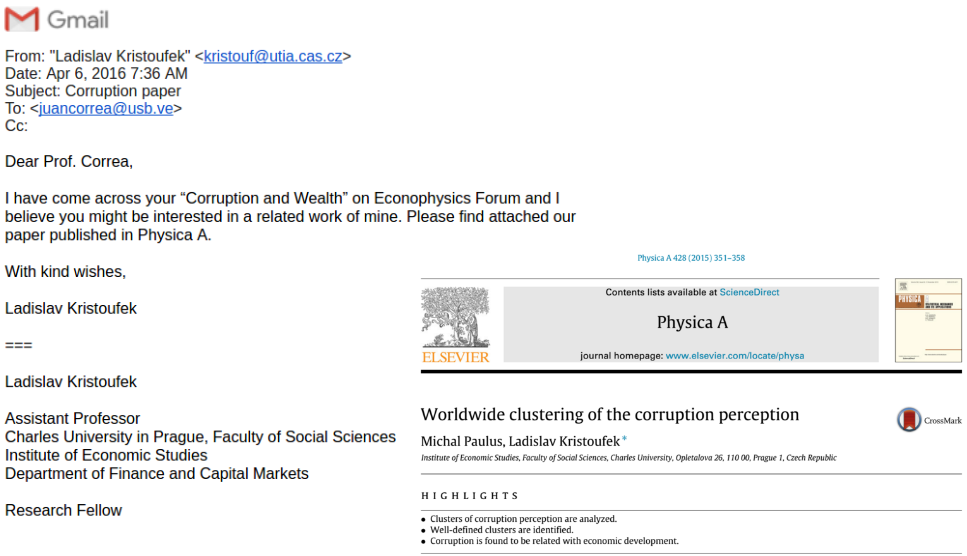
\includegraphics[width=0.91\textwidth]{c3}
 \end{figure}
\end{frame}

\subsection{Consumismo Ideológico en Elecciones Colombianas}
\begin{frame}{Consumismo Ideológico en Elecciones Colombianas}
\tiny{\textcolor{blue}{\url{https://www.liebertpub.com/doi/pdfplus/10.1089/cyber.2016.0402}}}
\begin{figure}
\centering
 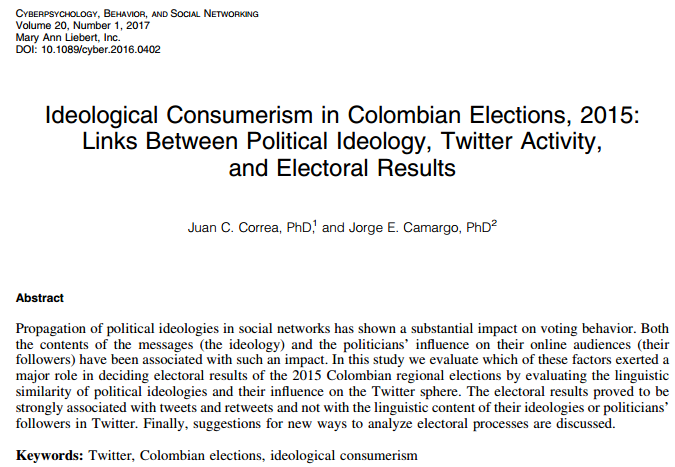
\includegraphics[width=.85\textwidth]{paper}
 \end{figure}
\end{frame}

\begin{frame}{Consumismo Ideológico en Elecciones Colombianas}
52 candidatos a gobernadores; 52 colecciones de tweets; 69202 tweets; número promedio de tweets por candidato; número promedio de retweets por tweet por candidato; ideología política; similaridad lingüística entre ideologías; resultados electorales (número de votos recibidos).
\begin{figure}
\centering
 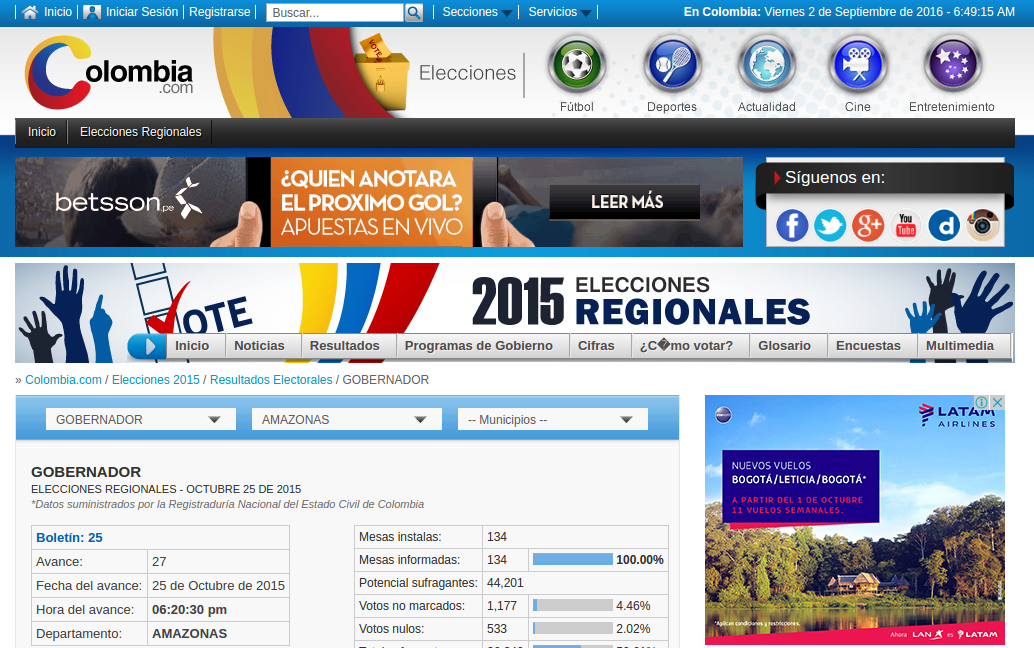
\includegraphics[width=0.6\textwidth]{art3}
 \end{figure}
\end{frame}

\begin{frame}{Consumismo Ideológico en Elecciones Colombianas}
\begin{figure}
\centering
 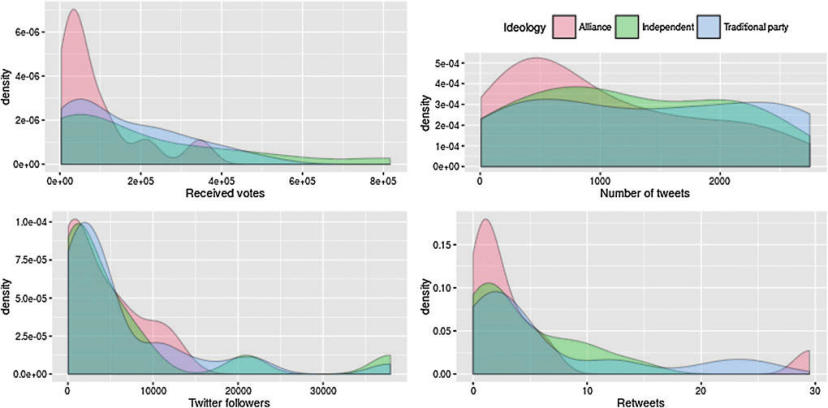
\includegraphics[width=1\textwidth]{results2}
 \end{figure}
\end{frame}

\begin{frame}{Consumismo Ideológico en Elecciones Colombianas}
\begin{figure}
\centering
 
\includegraphics[width=1\textwidth]{R1}
 \end{figure}
\end{frame}


\begin{frame}{Consumismo Ideológico en Elecciones Colombianas}
\begin{figure}
\centering
 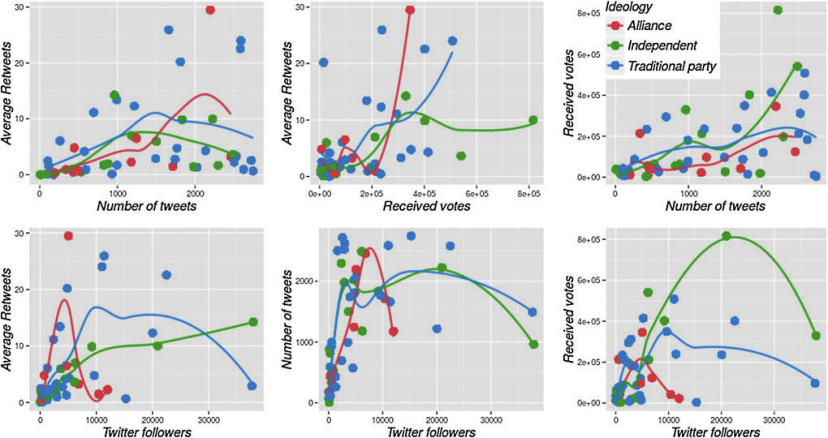
\includegraphics[width=0.96\textwidth]{R3}
 \end{figure}
\end{frame}

\section{Un ejemplo guiado en Rstudio Cloud}
\begin{frame}{Un ejemplo guiado en Rstudio Cloud}
Descargar los datos y el script para reproducir los gráficos incluidos en el artículo de consumismo ideológico en elecciones colombianas.
\begin{figure}
\centering
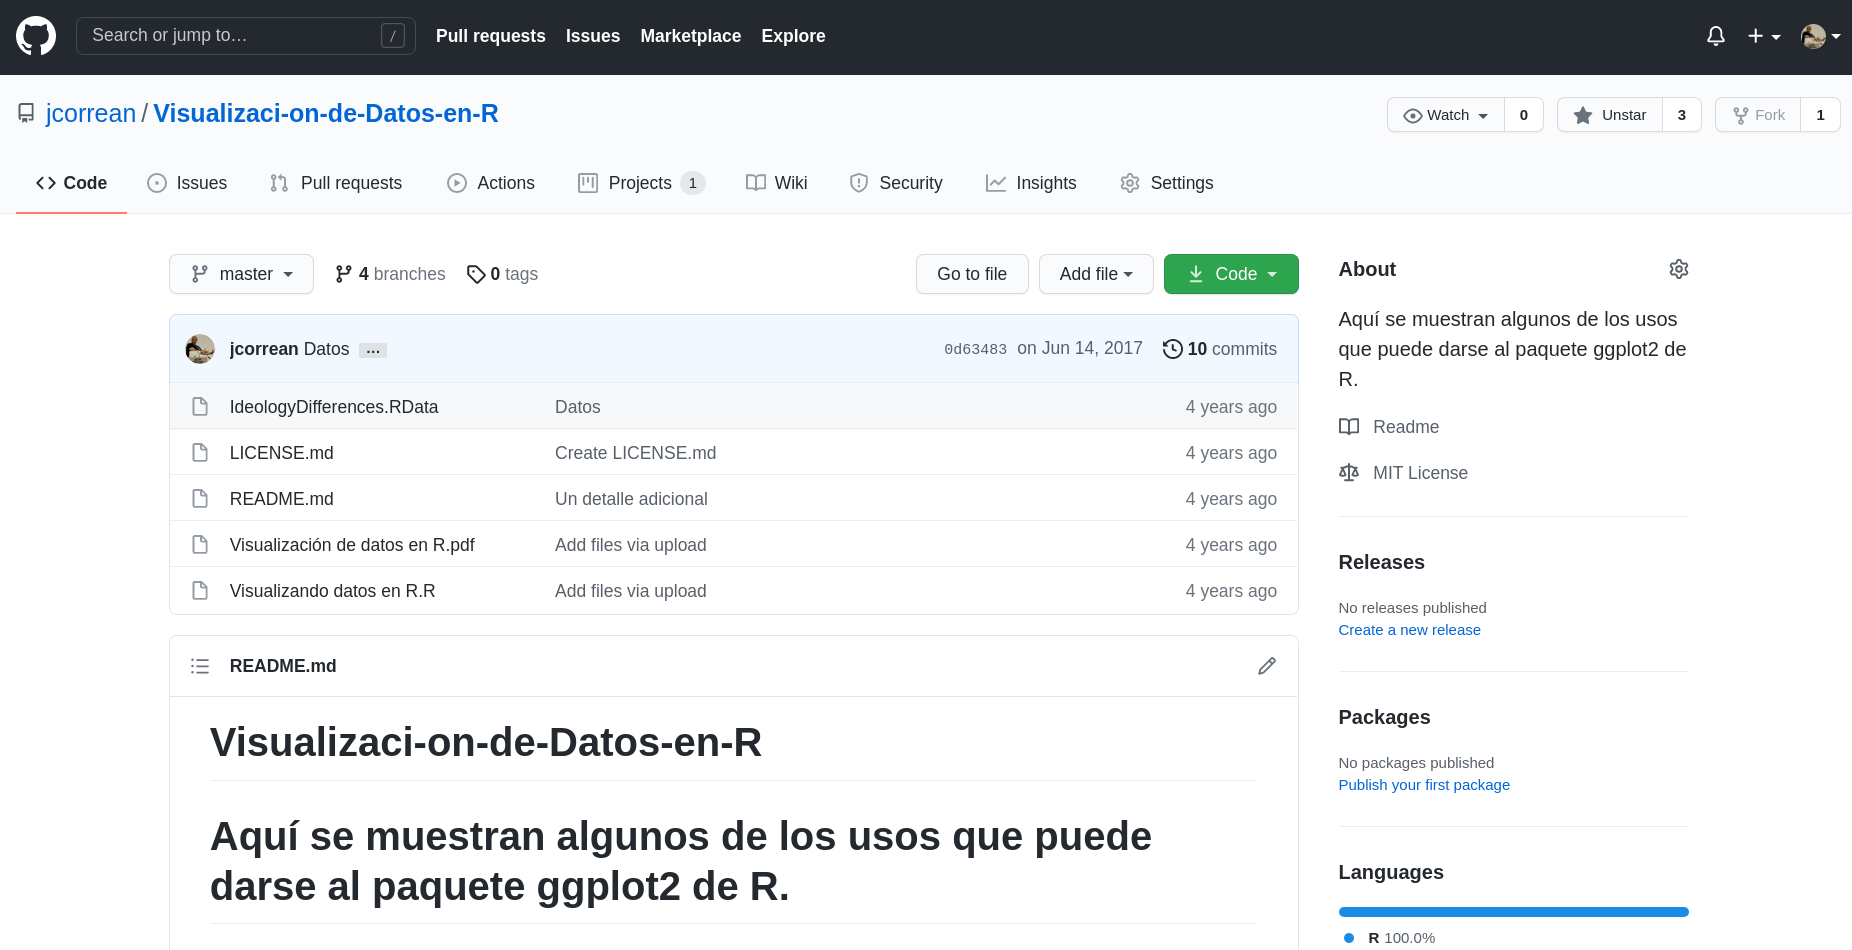
\includegraphics[width=0.8\textwidth]{GitHub.png}
\end{figure}
\textcolor{blue}{\url{https://github.com/jcorrean/Visualizaci-on-de-Datos-en-R}}
\end{frame}

\begin{frame}{Un ejemplo guiado en Rstudio Cloud}
Crear una cuenta en Rstudio Cloud
\begin{figure}
\centering
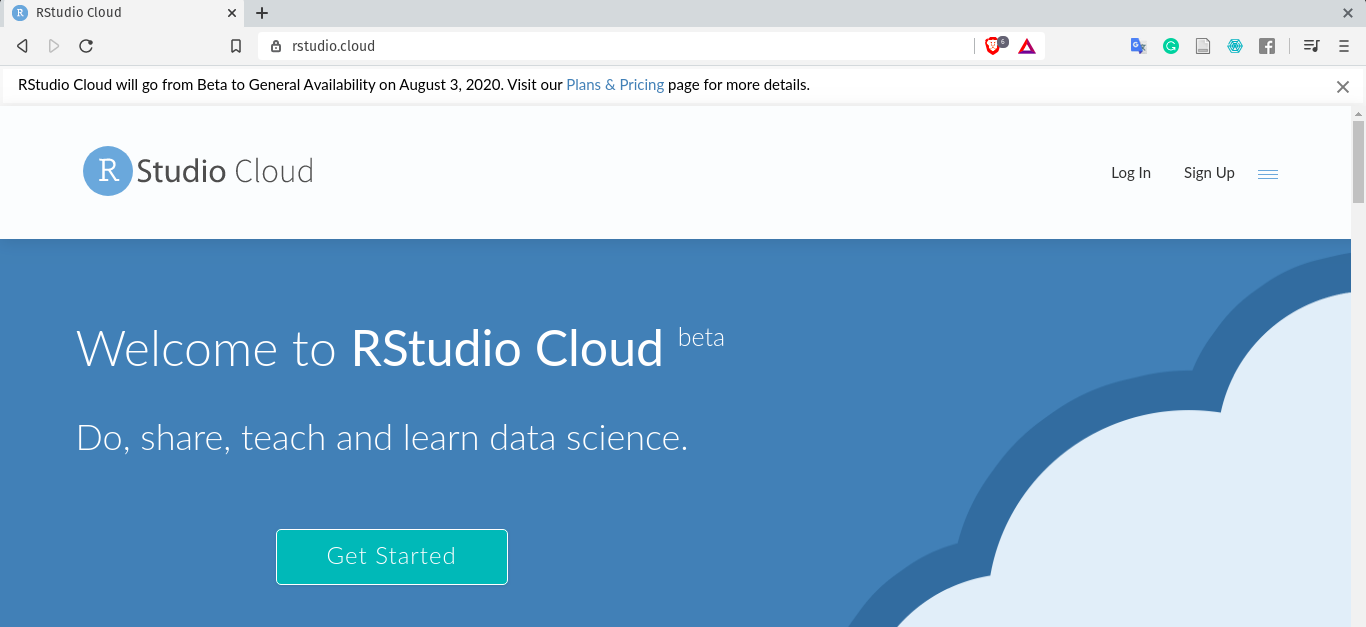
\includegraphics[width=0.9\textwidth]{RstudioCloud.png}
\end{figure}
\textcolor{blue}{\url{https://rstudio.cloud/}}
\end{frame}

\begin{frame}{Un ejemplo guiado en Rstudio Cloud}
\begin{figure}
\centering
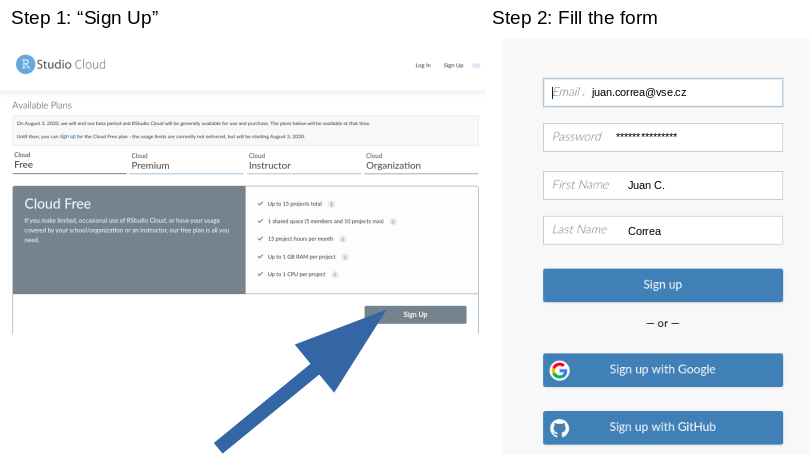
\includegraphics[width=1\textwidth]{RstudioAccount.png}
\end{figure}  
\end{frame}

\begin{frame}{Un ejemplo guiado en Rstudio Cloud}
Renombrar el workspace como ``VisualizacióndeDatosenR'' 
\begin{figure}
\centering
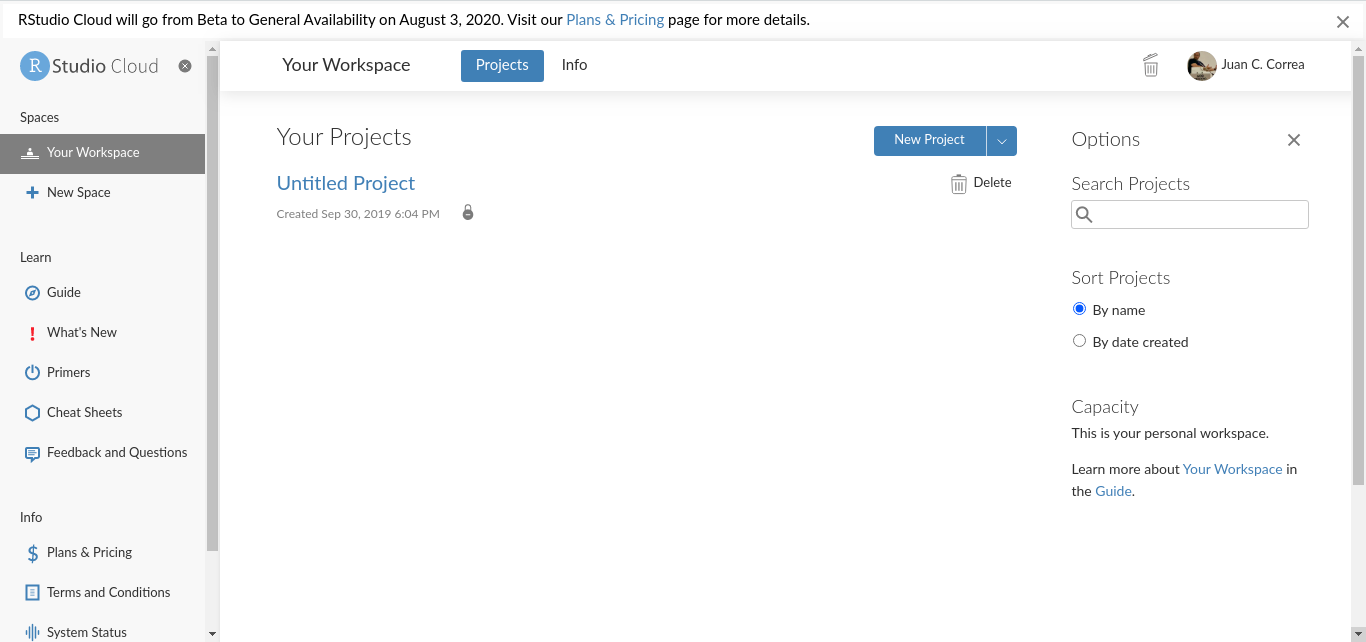
\includegraphics[width=1\textwidth]{PantallaInicial.png}
\end{figure}  
\end{frame}

\begin{frame}{Un ejemplo guiado en Rstudio Cloud}
\begin{figure}
\centering
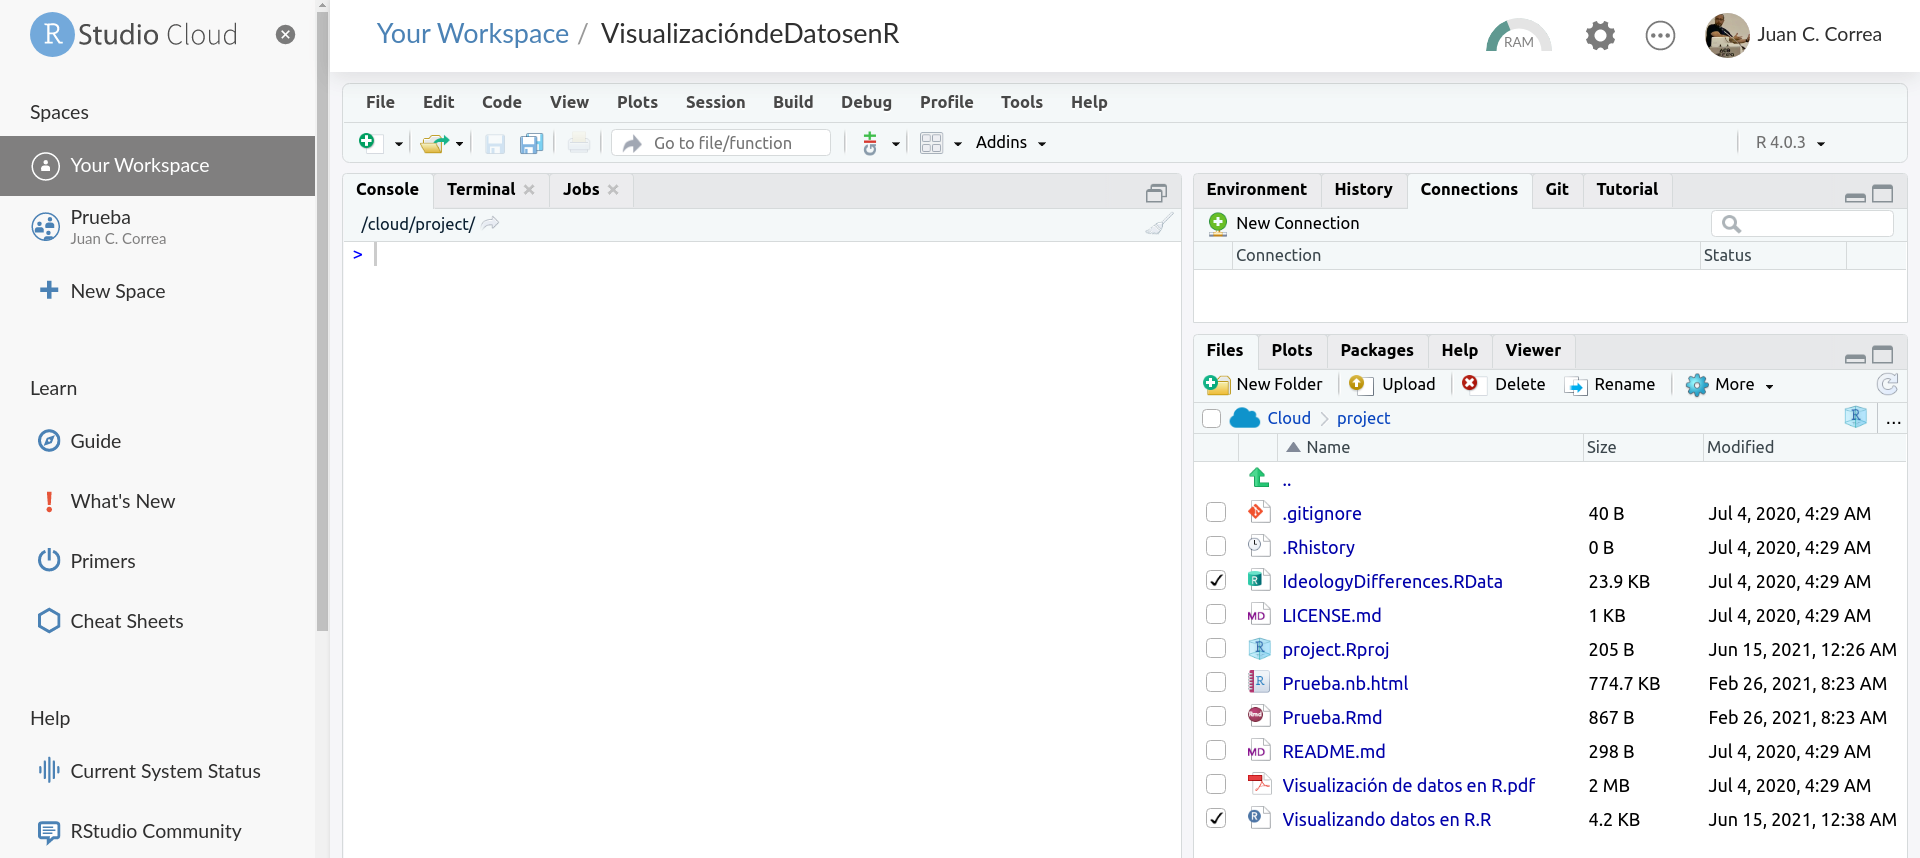
\includegraphics[width=1\textwidth]{PantallaModificada.png}
\end{figure}  
\end{frame}

\begin{frame}{Un ejemplo guiado en Rstudio Cloud}
Clic en el ícono de la carpeta amarilla (arriba a la izquierda, debajo del menú Edit).
\begin{figure}
\centering
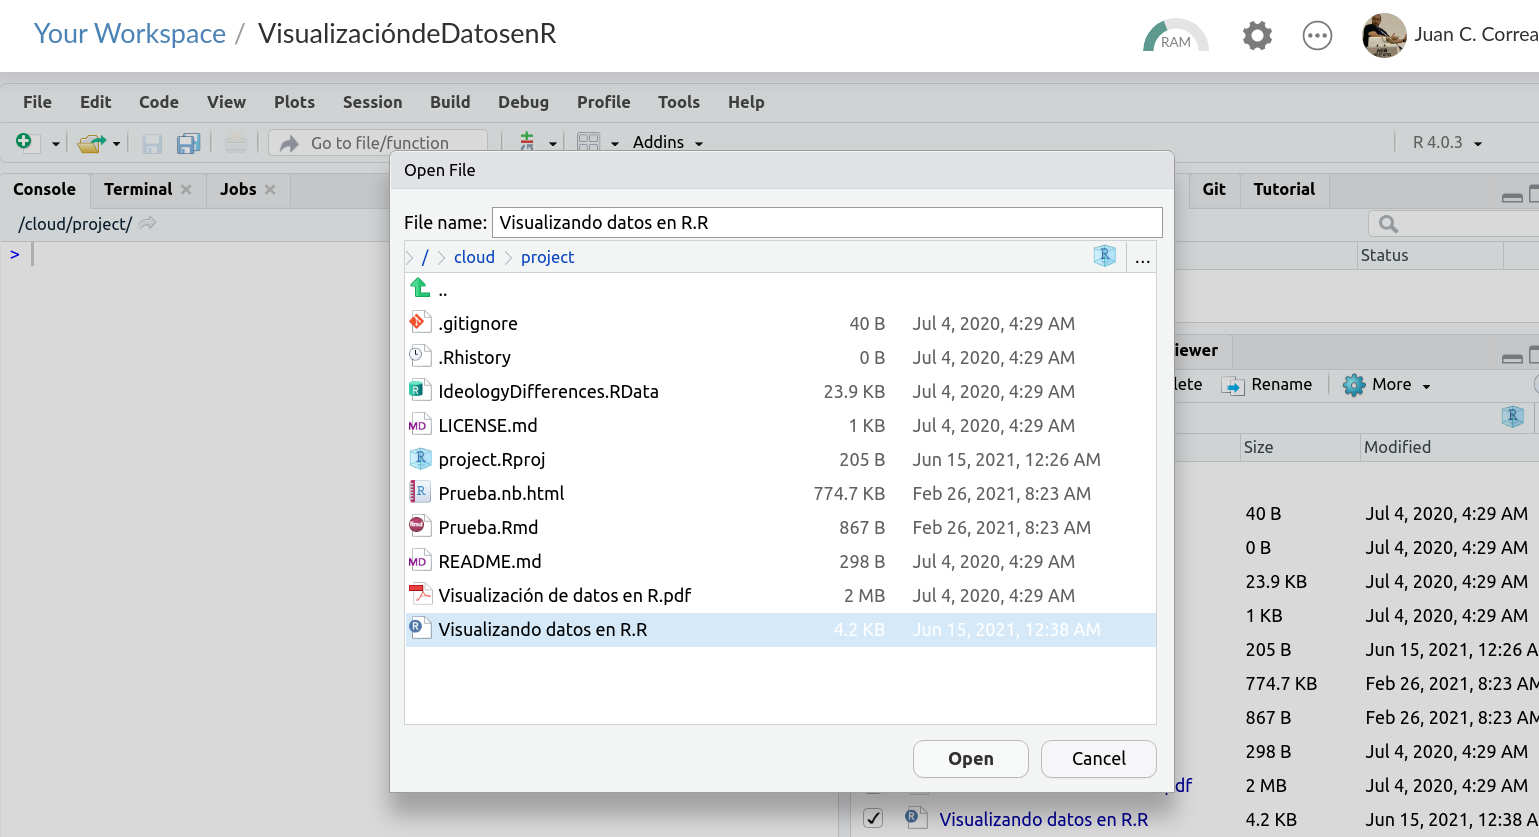
\includegraphics[width=.7\textwidth]{AbrirScript.png}
\end{figure}  
Clic en el archivo ``Visualizando datos en R.R'' y luego en el boton Open.
\end{frame}

\begin{frame}{Un ejemplo guiado en Rstudio Cloud}
Clic en el ícono de la carpeta amarilla (arriba a la izquierda, debajo del menú Edit).
\begin{figure}
\centering
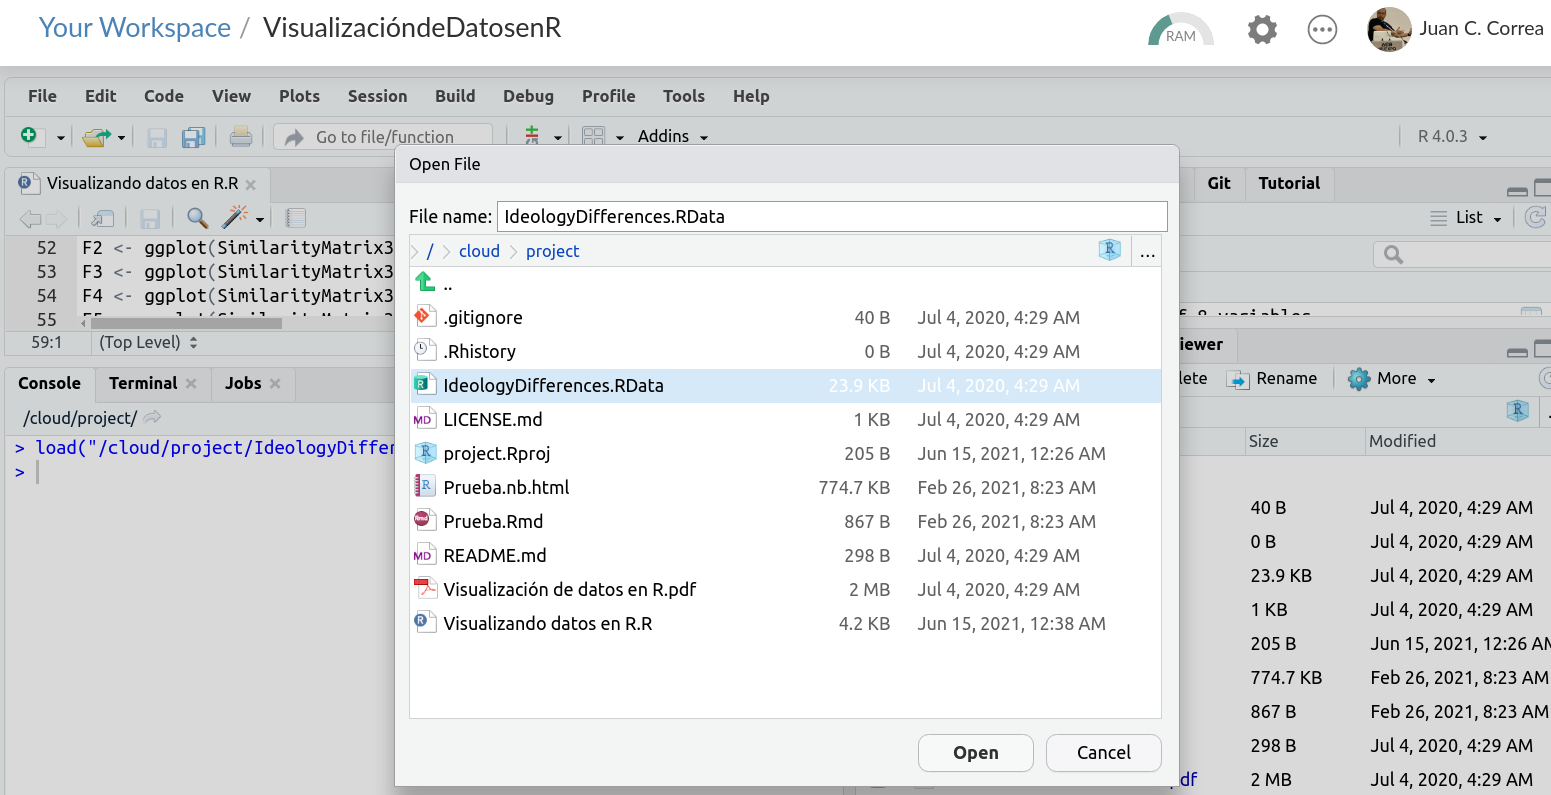
\includegraphics[width=.7\textwidth]{AbrirDatos.png}
\end{figure}  
Clic en el archivo ``IdeologyDifferences.RData'' y luego en el boton Open.
\end{frame}

\begin{frame}{Un ejemplo guiado en Rstudio Cloud}
\begin{figure}
\centering
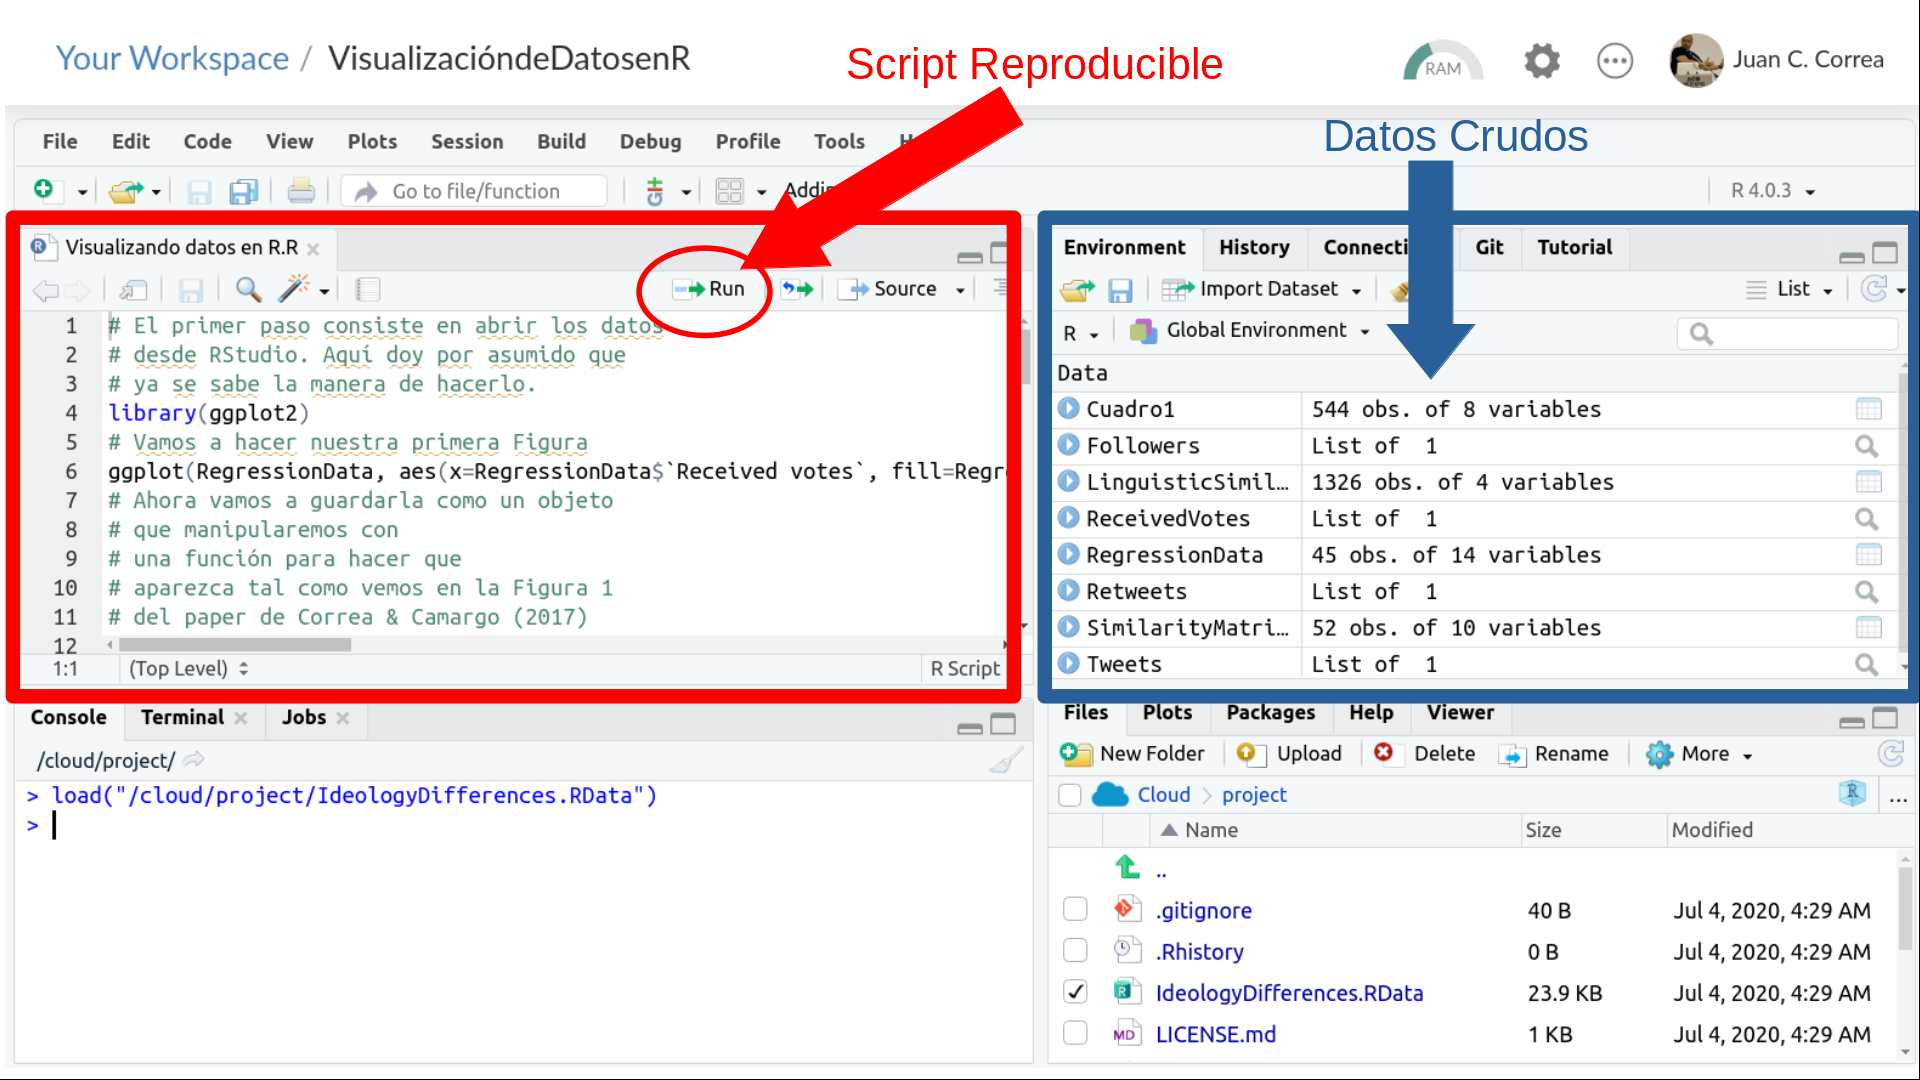
\includegraphics[width=1\textwidth]{Listo.png}
\end{figure}  
Clic en el boton Run dentro del recuadro rojo para obtener los mismos gráficos.
\end{frame}

\section{Recomendaciones}
\begin{frame}{Recomendaciones}
\begin{figure}
\centering

\includegraphics[width=.9\textwidth]{Simple.jpeg}
\end{figure}  
\end{frame}

\begin{frame}{Recomendaciones}
\begin{figure}
\centering

\includegraphics[width=.9\textwidth]{Chupitos.png}
\end{figure}  
\textcolor{blue}{\url{https://youtu.be/Qdz7V94lhI0}}
\end{frame}

\end{document}